\chapter{Discussion}\label{chap:discussion}


\section{Design Choices}

One-hole contexts vs multi-hole contexts (possible using extended signature).

Casteran's ordinals in Veblen nf vs Mamane's set-theoretic ordinals vs tree
ordinals.

Bisimilarity in steps.

The embedding relation and order on ordinals by Hancock, are there other
choices?

Positions are just lists (using option types) versus a safe position
type parameterised by a term.

Coinductive terms versus functions from lists of positions.

Why \Coq?


\subsection{Guardedness}\label{sub:guardedness}

% TODO: cite coquand, gimenez

Objects in a coinductive type may be infinite (i.e.\ contain an infinite
amount of constructors). However, in order to guarantee productivity,
definitions of such objects are required by \Coq to be in \emph{guarded}
form \citep{gimenez-94}. A corecursive definition in guarded form
satisfies two (syntactical) conditions. First, every corecursive call
must occur inside at least one constructor (of the same coinductive
type). Second, every corecursive call may only occur inside
abstractions or constructors (of the same coinductive
type).\footnote{To be more precise, the corecursive call is also
  allowed to occur inside \coqdockw{match} constructs and other
  corecursive definitions.}

In the \coqref{Term.term}{\coqdocinductive{term}} definition, we use a vector
type, parameterised by the type of its element and its size. Naturally, one
would implement a vector type in \Coq inductively, as for example has been
done in the standard library.
\begin{singlespace}
\begin{coqdoccode}
\coqdocnoindent
\coqdockw{Inductive} \coqdef{Bvector.vector}{vector}{\coqdocinductive{vector}}
(\coqdocvar{A} : \coqdockw{Type}) :
\coqexternalref{http://coq.inria.fr/stdlib/Coq.Init.Datatypes}{nat}{\coqdocinductive{nat}}
\ensuremath{\rightarrow} \coqdockw{Type} :=\coqdoceol
\coqdocindent{1.00em}
\ensuremath{|} \coqdef{Bvector.Vnil}{Vnil}{\coqdocconstructor{Vnil}}  :
\coqref{Bvector.vector}{\coqdocinductive{vector}} \coqdocvariable{A} 0\coqdoceol
\coqdocindent{1.00em}
\ensuremath{|} \coqdef{Bvector.Vcons}{Vcons}{\coqdocconstructor{Vcons}} :
\coqdocvariable{A} \ensuremath{\rightarrow} \ensuremath{\forall} \coqdocvar{n},
\coqref{Bvector.vector}{\coqdocinductive{vector}} \coqdocvariable{A}
\coqdocvariable{n} \ensuremath{\rightarrow}
\coqref{Bvector.vector}{\coqdocinductive{vector}} \coqdocvariable{A}
(\coqexternalref{http://coq.inria.fr/stdlib/Coq.Init.Datatypes}{S}{\coqdocconstructor{S}}
\coqdocvariable{n}).\coqdoceol
\end{coqdoccode}
\end{singlespace}

Now consider the following trivial example of a basic operation on terms by
corecursive traversal.
\begin{singlespace}
\begin{coqdoccode}
\coqdocnoindent
\coqdockw{CoFixpoint} \coqdef{Term.id}{id}{\coqdocdefinition{id}}
(\coqdocvar{t} : \coqref{Term.term}{\coqdocinductive{term}}) :
\coqref{Term.term}{\coqdocinductive{term}} :=\coqdoceol
\coqdocindent{1.00em}
\coqdockw{match} \coqdocvariable{t} \coqdockw{with}\coqdoceol
\coqdocindent{1.00em}
\ensuremath{|} \coqref{Term.Var}{\coqdocconstructor{Var}} \coqdocvar{x}
\ensuremath{\Rightarrow} \coqref{Term.Var}{\coqdocconstructor{Var}}
\coqdocvariable{x}\coqdoceol
\coqdocindent{1.00em}
\ensuremath{|} \coqref{Term.Fun}{\coqdocconstructor{Fun}} \coqdocvar{f}
\coqdocvar{args} \ensuremath{\Rightarrow}
\coqref{Term.Fun}{\coqdocconstructor{Fun}} \coqdocvariable{f}
(\coqdocdefinition{vmap} \coqref{Term.id}{\coqdocdefinition{id}}
\coqdocvariable{args})\coqdoceol
\coqdocindent{1.00em}
\coqdockw{end}.\coqdoceol
\end{coqdoccode}
\end{singlespace}
This definition is ill-formed, since the corecursive call to
\coqref{Term.id}{\coqdocdefinition{id}} is not guarded.\footnote{The call to
  \coqref{Term.id}{\coqdocdefinition{id}} is hidden inside
  \coqdocdefinition{vmap}, which is defined by recursion on the vector
  \coqdocvariable{args}.}
We define a recursive type of vectors as an alternative to the inductive type:
\begin{singlespace}
\begin{coqdoccode}
\coqdocnoindent
\coqdockw{Inductive} \coqdef{Vector.Fin}{Fin}{\coqdocinductive{Fin}} :
\coqexternalref{http://coq.inria.fr/stdlib/Coq.Init.Datatypes}{nat}{\coqdocinductive{nat}}
\ensuremath{\rightarrow} \coqdockw{Type} :=\coqdoceol
\coqdocindent{1.00em}
\ensuremath{|} \coqdef{Vector.First}{First}{\coqdocconstructor{First}} :
\ensuremath{\forall} \coqdocvar{n}, \coqref{Vector.Fin}{\coqdocinductive{Fin}}
(\coqexternalref{http://coq.inria.fr/stdlib/Coq.Init.Datatypes}{S}{\coqdocconstructor{S}}
\coqdocvariable{n})\coqdoceol
\coqdocindent{1.00em}
\ensuremath{|} \coqdef{Vector.Next}{Next}{\coqdocconstructor{Next}}  :
\ensuremath{\forall} \coqdocvar{n}, \coqref{Vector.Fin}{\coqdocinductive{Fin}}
\coqdocvariable{n} \ensuremath{\rightarrow}
\coqref{Vector.Fin}{\coqdocinductive{Fin}}
(\coqexternalref{http://coq.inria.fr/stdlib/Coq.Init.Datatypes}{S}{\coqdocconstructor{S}}
\coqdocvariable{n}).\coqdoceol
\coqdocemptyline
\coqdocnoindent
\coqdockw{Definition}
\coqdef{Vector.vector}{vector}{\coqdocdefinition{vector}} (\coqdocvar{A} :
\coqdockw{Type}) (\coqdocvar{n} :
\coqexternalref{http://coq.inria.fr/stdlib/Coq.Init.Datatypes}{nat}{\coqdocinductive{nat}})
:= \coqref{Vector.Fin}{\coqdocinductive{Fin}} \coqdocvariable{n}
\ensuremath{\rightarrow} \coqdocvariable{A}.\coqdoceol
\end{coqdoccode}
\end{singlespace}
% TODO: explain this vector type
This makes for a definition of \coqref{Vector.vmap}{\coqdocdefinition{vmap}}
that is just an abstraction, and therefore solves the guardedness problem in
\coqref{Term.id}{\coqdocdefinition{id}}.
\begin{singlespace}
\begin{coqdoccode}
\coqdocnoindent
\coqdockw{Definition} \coqdef{Vector.vmap}{vmap}{\coqdocdefinition{vmap}}
\coqdocvar{A} \coqdocvar{B} (\coqdocvar{f} :
\coqdocvariable{A} \ensuremath{\rightarrow} \coqdocvariable{B}) \coqdocvar{n}
: \coqref{Vector.vector}{\coqdocdefinition{vector}} \coqdocvariable{A}
\coqdocvariable{n} \ensuremath{\rightarrow}
\coqref{Vector.vector}{\coqdocdefinition{vector}} \coqdocvariable{B}
\coqdocvariable{n} :=\coqdoceol
\coqdocindent{1.00em}
\coqdockw{fun} \coqdocvar{v} \coqdocvar{i} \ensuremath{\Rightarrow}
\coqdocvariable{f} (\coqdocvariable{v} \coqdocvariable{i}).\coqdoceol
\end{coqdoccode}
\end{singlespace}


\subsection{The Positivity Condition}\label{sub:positivity}

\Coq restricts inductive definitions to those that satisfy the
\emph{positivity condition}. The reason for this is that definitions
that fail this (syntactic) criterion may lead to an inconsistent
  system. For a precise definition of positivity, consult
  \citetalias[Section 4.5.3]{coq-refman-09}.

Consider again the definition of rewrite sequences from
Section~\ref{sec:seq}. A more natural way to define the type of the
\coqref{Rewriting.Lim}{\coqdocconstructor{Lim}} constructor might be
by using a $\Sigma$-type instead of a separate function for the target
terms of the branches.
\begin{singlespace}
\begin{coqdoccode}
\coqdocindent{1.00em}
\ensuremath{|} \coqdocconstructor{Lim} :
\ensuremath{\forall} \coqdocvar{s} \coqdocvar{t}
(\coqdocvar{f} :
\coqexternalref{http://coq.inria.fr/stdlib/Coq.Init.Datatypes}{nat}{\coqdocinductive{nat}}
\ensuremath{\rightarrow} \{ \coqdocvar{t'} : \coqref{Term.term}{\coqdocinductive{term}}
\& \coqdocvar{s}
\coqref{Rewriting.sequence}{$\rewrites_\mathcal{R}$}
\coqdocvariable{t'} \}),\coqdoceol
\coqdocindent{5.00em}
\coqref{Rewriting.converges}{\coqdocdefinition{converges}}
(\coqdockw{fun} \coqdocvar{n} \ensuremath{\Rightarrow}
\coqexternalref{http://coq.inria.fr/stdlib/Coq.Init.Specif}{projT1}{\coqdocdefinition{projT1}}
(\coqdocvariable{f} \coqdocvariable{n})) \coqdocvariable{t}
$\rightarrow$ (\coqdocvariable{s}
\coqref{Rewriting.sequence}{$\rewrites_\mathcal{R}$}
\coqdocvariable{t})\coqdoceol
\end{coqdoccode}
\end{singlespace}
However, this type definition does not satisfy the positivity
condition and therefore we cannot use it. We feel that the definition
from Section~\ref{sec:seq}, which does satisfy the condition, models
our intentions adequately.


\subsection{Convergence of Rewrite Sequences}\label{sub:convergence}

The inductively defined rewrite sequences from Section~\ref{sec:seq}
are not necessarily (weakly) convergent. A rewrite sequence of limit
length satisfies the condition that the target terms of the
\coqref{Rewriting.Lim}{\coqdocconstructor{Lim}} branches converge but
this is obviously too weak to establish convergence of the rewrite
sequence itself.

The depths of the rewrite steps are not considered at all in our
formalisation and therefore it obviously does not implement strong
convergence.

We consider an example of a rewrite sequence that satisfies the
inductive definition but is not weakly convergent. Let $A$ be a
constant and $B, C, D$ unary function symbols. We use the following
three rewrite rules:
\begin{align*}
  \rho_1 \, : \, A \to B(A) \qquad \qquad
  \rho_2 \, : \, C(x) \to D(x) \qquad \qquad
  \rho_3 \, : \, D(x) \to C(x)
\end{align*}
The term $C(A)$ rewrites in $\omega$ many $\rho_1$-steps to
$C(B^\omega)$.
\begin{center}
{\footnotesize\begin{tikzpicture}[node distance=50pt]
\tikzstyle{level}=[level distance=20pt,sibling distance=22pt]
\node (a) {$C$} child { node {$A$} };
\node (b) [right of=a] {$C$} child { node {$B$} child { node {$A$} } };
\node (c) [right of=b] {$C$} child { node {$B$} child { node {$B$}
    child { node {$A$} } } };
\node (d) [right of=c,node distance=80pt] {$C$} child { node {$B$}
  child { node {$B$} child { node {$B$} child { node[below=-6pt]
        {\scriptsize$\vdots$} } } } };
\path (a) -- (b) node[midway,below=-1pt] {$\rightarrow_{\rho_1}$};
\path (b) -- (c) node[midway,below=-1pt] {$\rightarrow_{\rho_1}$};
\path (c) -- (d) node[midway,below=-1pt] {$\rightarrow_{\rho_1} \quad \cdots$};
\end{tikzpicture}}
\end{center}\vspace{-0.8\baselineskip}
We modify this rewrite sequence such that in between every two
$\rho_1$-steps, the root symbol $C$ is changed to $D$ and back to
$C$. The resulting rewrite sequence does not have a limit and is not
weakly convergent.
\begin{center}
{\footnotesize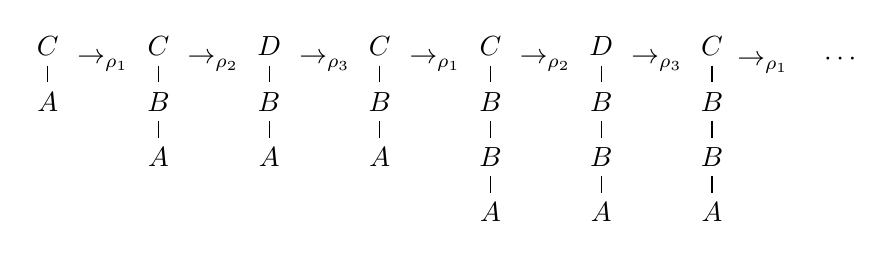
\begin{tikzpicture}[node distance=40pt]
\tikzstyle{level}=[level distance=20pt,sibling distance=22pt]
\node (a) {$C$} child { node {$A$} };
\node (a') [right of=a] {$C$} child { node {$B$} child { node {$A$} } };
\node (a'') [right of=a'] {$D$} child { node {$B$} child { node {$A$} } };
\node (b) [right of=a''] {$C$} child { node {$B$} child { node {$A$} } };
\node (b') [right of=b] {$C$} child { node {$B$} child { node {$B$}
    child { node {$A$} } } };
\node (b'') [right of=b'] {$D$} child { node {$B$} child { node {$B$}
    child { node {$A$} } } };
\node (c) [right of=b''] {$C$} child { node {$B$} child { node {$B$}
    child { node {$A$} } } };
\node (d) [right of=c] {};
\path (a) -- (a') node[midway,below=-1pt] {$\rightarrow_{\rho_1}$};
\path (a') -- (a'') node[midway,below=-1pt] {$\rightarrow_{\rho_2}$};
\path (a'') -- (b) node[midway,below=-1pt] {$\rightarrow_{\rho_3}$};
\path (b) -- (b') node[midway,below=-1pt] {$\rightarrow_{\rho_1}$};
\path (b') -- (b'') node[midway,below=-1pt] {$\rightarrow_{\rho_2}$};
\path (b'') -- (c) node[midway,below=-1pt] {$\rightarrow_{\rho_3}$};
\path (c) -- (d) node[pos=.8,below=-1pt] {$\rightarrow_{\rho_1} \quad \cdots$};
\end{tikzpicture}}
\end{center}\vspace{-0.8\baselineskip}
We can define this rewrite sequence as the limit of
$(\varphi_n)_{n \in \mathbb{N}}$, where $\concat$ denotes
concatenation of rewrite sequences:
\begin{align*}
  \varphi_0 \, &: \, \mbox{\emph{empty}}\\
  \varphi_{n + 1} \, &: \, \varphi_n \concat C(B^n(A)) \to_{\rho_1}
  C(B^{n + 1}(A)) \to_{\rho_2} D(B^{n + 1}(A)) \to_{\rho_3} C(B^{n +
    1}(A))
\end{align*}
The target terms $C(B^{n + 1}(A))$ converge to $C(B^\omega)$ and this
construction can thus be used with our inductive definition of rewrite
sequences, where we take $\varphi_n$ to be the $n$\textsuperscript{th}
branch of the \coqref{Rewriting.Lim}{\coqdocconstructor{Lim}}
constructor.

% $\varphi_n$ is the prefix of length $3n$.

% 'stuttering convergence'
% convergence with hiccups
% the difference between t_n and the limit t is oscillating

It is not clear to us whether there is some natural translation of the
convergence conditions to our formalisation. Without such a
translation, we feel our definitions are not satisfactory.

For completeness we include a (not so natural) translation of
convergence, but we were not able to use this in our development. Even
proving the simplest of rewrite sequences to satisfy these definitions
seemed over our head.
\begin{singlespace}
\begin{coqdoccode}
\coqdocnoindent
\coqdockw{Fixpoint}
\coqdef{Rewriting.weaklyconvergent}{weakly\_convergent}{\coqdocdefinition{weakly\_convergent}}
\coqdocvar{s} \coqdocvar{t} (\coqdocvar{$\varphi$} : \coqdocvar{s} \coqref{Rewriting.sequence}{$\rewrites_\mathcal{R}$} \coqdocvar{t}) : \coqdockw{Prop}
:=\coqdoceol
\coqdocindent{1.00em}
\coqdockw{match} \coqdocvariable{$\varphi$} \coqdockw{with}\coqdoceol
\coqdocindent{1.00em}
\ensuremath{|} \coqref{Rewriting.Nil}{\coqdocconstructor{Nil}}
\coqdocvar{\_}          \ensuremath{\Rightarrow}
\coqexternalref{http://coq.inria.fr/stdlib/Coq.Init.Logic}{True}{\coqdocinductive{True}}\coqdoceol
\coqdocindent{1.00em}
\ensuremath{|} \coqref{Rewriting.Cons}{\coqdocconstructor{Cons}}
\coqdocvar{\_} \coqdocvar{\_} \coqdocvar{$\psi$} \coqdocvar{\_}
\coqdocvar{\_} \ensuremath{\Rightarrow}
\coqref{Rewriting.weaklyconvergent}{\coqdocdefinition{weakly\_convergent}}
\coqdocvariable{$\psi$}\coqdoceol
\coqdocindent{1.00em}
\ensuremath{|} \coqref{Rewriting.Lim}{\coqdocconstructor{Lim}}
\coqdocvar{\_} \coqdocvar{\_} \coqdocvar{f} \coqdocvar{t}
\coqdocvar{\_}  \ensuremath{\Rightarrow}\coqdoceol
\coqdocindent{2.00em}
(\ensuremath{\forall} \coqdocvar{n},
\coqref{Rewriting.weaklyconvergent}{\coqdocdefinition{weakly\_convergent}}
(\coqdocvariable{f} \coqdocvariable{n})) \ensuremath{\land}\coqdoceol
\coqdocindent{2.00em}
\ensuremath{\forall} \coqdocvar{d}, \ensuremath{\exists}
\coqdocvar{n}, \ensuremath{\forall} \coqdocvar{$\iota$},\coqdoceol
\coqdocindent{3.00em}
\coqdocvariable{f} \coqdocvariable{n} \coqref{Rewriting.embed}{$\sqsubseteq$}
\coqdocvariable{$\varphi$}[\coqdocvariable{$\iota$}]$^\textsc{seq}$
\ensuremath{\rightarrow}\coqdoceol
\coqdocindent{3.00em}
\coqdocvariable{$\varphi$}[\coqdocvariable{$\iota$}]$^\textsc{l}$
\coqref{TermEquality.termequpto}{\equpto{\coqdocvariable{d}}}
\coqdocvariable{t}\coqdoceol
\coqdocindent{1.00em}
\coqdockw{end}.\coqdoceol
\coqdocemptyline
\coqdocnoindent
\coqdockw{Fixpoint}
\coqdef{Rewriting.stronglyconvergent}{strongly\_convergent}{\coqdocdefinition{strongly\_convergent}}
\coqdocvar{s} \coqdocvar{t} (\coqdocvar{$\varphi$} : \coqdocvar{s} \coqref{Rewriting.sequence}{$\rewrites_\mathcal{R}$} \coqdocvar{t}) : \coqdockw{Prop}
:=\coqdoceol
\coqdocindent{1.00em}
\coqdockw{match} \coqdocvariable{$\varphi$} \coqdockw{with}\coqdoceol
\coqdocindent{1.00em}
\ensuremath{|} \coqref{Rewriting.Nil}{\coqdocconstructor{Nil}}
\coqdocvar{\_}          \ensuremath{\Rightarrow}
\coqexternalref{http://coq.inria.fr/stdlib/Coq.Init.Logic}{True}{\coqdocinductive{True}}\coqdoceol
\coqdocindent{1.00em}
\ensuremath{|} \coqref{Rewriting.Cons}{\coqdocconstructor{Cons}}
\coqdocvar{\_} \coqdocvar{\_} \coqdocvar{$\psi$} \coqdocvar{\_}
\coqdocvar{\_} \ensuremath{\Rightarrow}
\coqref{Rewriting.stronglyconvergent}{\coqdocdefinition{strongly\_convergent}}
\coqdocvariable{$\psi$}\coqdoceol
\coqdocindent{1.00em}
\ensuremath{|} \coqref{Rewriting.Lim}{\coqdocconstructor{Lim}}
\coqdocvar{\_} \coqdocvar{\_} \coqdocvar{f} \coqdocvar{t}
\coqdocvar{\_}  \ensuremath{\Rightarrow}\coqdoceol
\coqdocindent{2.00em}
(\ensuremath{\forall} \coqdocvar{n},
\coqref{Rewriting.stronglyconvergent}{\coqdocdefinition{strongly\_convergent}}
(\coqdocvariable{f} \coqdocvariable{n})) \ensuremath{\land}\coqdoceol
\coqdocindent{2.00em}
\ensuremath{\forall} \coqdocvar{d}, \ensuremath{\exists}
\coqdocvar{$\iota$}, \ensuremath{\forall} \coqdocvar{$\kappa$},\coqdoceol
\coqdocindent{3.00em}
\coqdocvariable{$\varphi$}[\coqdocvariable{$\iota$}]$^\textsc{seq}$
\coqref{Rewriting.embed}{$\sqsubseteq$}
\coqdocvariable{$\varphi$}[\coqdocvariable{$\kappa$}]$^\textsc{seq}$
\ensuremath{\rightarrow}\coqdoceol
\coqdocindent{3.00em}
\coqdocvariable{d} $\le$
\coqdocdefinition{depth}
\coqdocvariable{$\varphi$}[\coqdocvariable{$\kappa$}]$^\textsc{stp}$\coqdoceol
\coqdocindent{1.00em}
\coqdockw{end}.\coqdoceol
\end{coqdoccode}
\end{singlespace}
Strong convergence should include weak convergence.


\subsection{Representation of Rewrite Sequences}

TODO

Rewrite sequences can also be represented by partial functions from
ordinals to rewrite steps.

The problem is that comparing ordinals is not decidable. Non-trivial
rewrite sequences can then not be effectively constructed.

Consider a rewrite sequence of length $\lambda$. For every
ordinal $\alpha < \lambda$, the function representing this
rewrite sequence must produce a step. For a non-trivial rewrite
sequence, this means it has to decide, given an ordinal, what step to
produce. But it cannot do this in finite time if comparing ordinals is
not decidable.

Comparing ordinals less than to some given upper bound may be
decidable, so this would not be a problem if we construct rewrite
sequences of limited length. Another representation for the ordinals
might also help here, for example cantor normal forms where comparing
is decidable (?).

Motivated by the compression lemma, we could go even further and
restrict our representation to rewrite sequences of length $\le
\omega$. This is of course not a real option. Much of the theory could
not be developed with this representation (e.g. compression itself)
and many rewrite sequences are best represented with length $>
\omega$.

Versus our inductive definition.


\section{Discussion}

Our representation feels natural, but the traditional convergence
definitions do not fit (easily). Maybe there are alternatives to our
embedding relation, or can we index the steps in a different way than
with predecessor indices.

Functions from ordinals to steps have other problems. They could be
investigated, especially using other ordinal representations such as
cantor normal form. But this is very not \Coq-like (partial functions
and algebraic representations).

Bvector vs Vector: we did not really hit the guardedness restriction, so we
could have used inductive Bvector. But it spells trouble later.
% TODO: in this text we *do* assume substitute is defined on infinite
% terms

TODO: additional remarks on productivity and guardedness restriction?

Related work.


\section{Conclusions}

TODO

Representation is original.

Original goal was compression.
